\documentclass[runningheads]{llncs}
%
\usepackage[T1]{fontenc}

\usepackage{amsfonts}

\usepackage{graphicx}

\usepackage{svg}

\usepackage{acronym}

\newcommand{\topic}{Approaches for finding sample pairs in contrastive learning}
\newcommand{\authorA}{Klara M. Gutekunst}

% If you use the hyperref package, please uncomment the following two lines
% to display URLs in blue roman font according to Springer's eBook style:
%\usepackage{color}
%\renewcommand\UrlFont{\color{blue}\rmfamily}
%\urlstyle{rm}
%
\begin{document}

\begin{acronym}

    \acro{nn}[NN]{Neural Network}

\end{acronym}
%
\title{\topic}
%
\titlerunning{\topic}

\author{\authorA}
%
\authorrunning{\authorA}

\institute{University of Kassel, Germany\\
\email{klara.gutekunst@student.uni-kassel.de}}
%
\maketitle         
%
% include: speed bonus, no reloads, but no nesting, forces page break after and before input
\begin{abstract}
    %The abstract should briefly summarize the contents of the paper in
    %150--250 words.
    % unsupervised learning
    Since labelled data is often scarce and expensive to obtain, 
    unsupervised learning has emerged as a powerful paradigm for training models without reliance on labelled data. 
    % SSL
    Within this domain, \acl{ssl} has gained significant attention, leveraging unlabelled data to generate labels.
    % CL
    A core concept within \acl{ssl} is \acl{cl}, which focuses on learning data representations by contrasting positive and negative sample pairs. 
    % representation learning
    The key idea is to encourage the model to map positive samples closer together in the representation space 
    while pushing negative samples farther apart.
    % hard positive/ negative pairs
    The selection of positive and negative pairs is of particular importance, 
    as challenging pairs present valuable learning opportunities for the model.
    % motivation
    A significant advantage of \acl{cl} in representation learning is its ability to capture the underlying structure of the data, 
    leading to the development of more robust and generalizable models.
    % this paper
    This review paper offers a comprehensive examination of various \acl{cl} approaches, 
    focusing on their foundational principles and the methods employed for pair selection, 
    while also providing a critical analysis of these techniques.
    
    \keywords{\acl{cl}  \and \acl{ssl} \and Hard sample mining.}
\end{abstract}

In order to explain why the proximity of generated samples to the anchor $x$ is relevant to the efficiency during training, 
one can consider a simple example in Euclidean space.
Imagine images as input to a \ac{nn}, which projects them onto $f_{\theta}(x) \in \mathbb{R}^d$, 
where $\theta$ are the parameters of the \ac{nn}.
The effect of the distance between the anchor $x$ and the positive $x^+$ (negative $x^-$) 
sample on the loss is visualized in \autoref{fig:hard_easy_samples_dist_effect_loss}.
Since difficult samples hold more (gradient) information, they have a higher loss value.
Hence, similar negative pairs ($x$, $x^-$) are considered hard \citet{robinson_contrastive_2021}, 
while distant positive pairs ($x$, $x^+$) are considered hard.

% \begin{figure}[h] % h = here, t = top, b = bottom, p = page of floats
%     \centering
%     \includesvg[width=300pt]{images/Hard_easy_samples_dist_effect_loss}
%     \caption{The impact of the distance between a generated sample and its anchor on the loss function.
%     Hard samples convey more (gradient) information than easy samples and thus, have a higher loss value.
%     While distant positive pairs are considered hard, for negative samples, small proximity ones are considered hard.}
%     \label{fig:hard_easy_samples_dist_effect_loss}
% \end{figure}

\begin{figure}[h] % h = here, t = top, b = bottom, p = page of floats
    \centering
    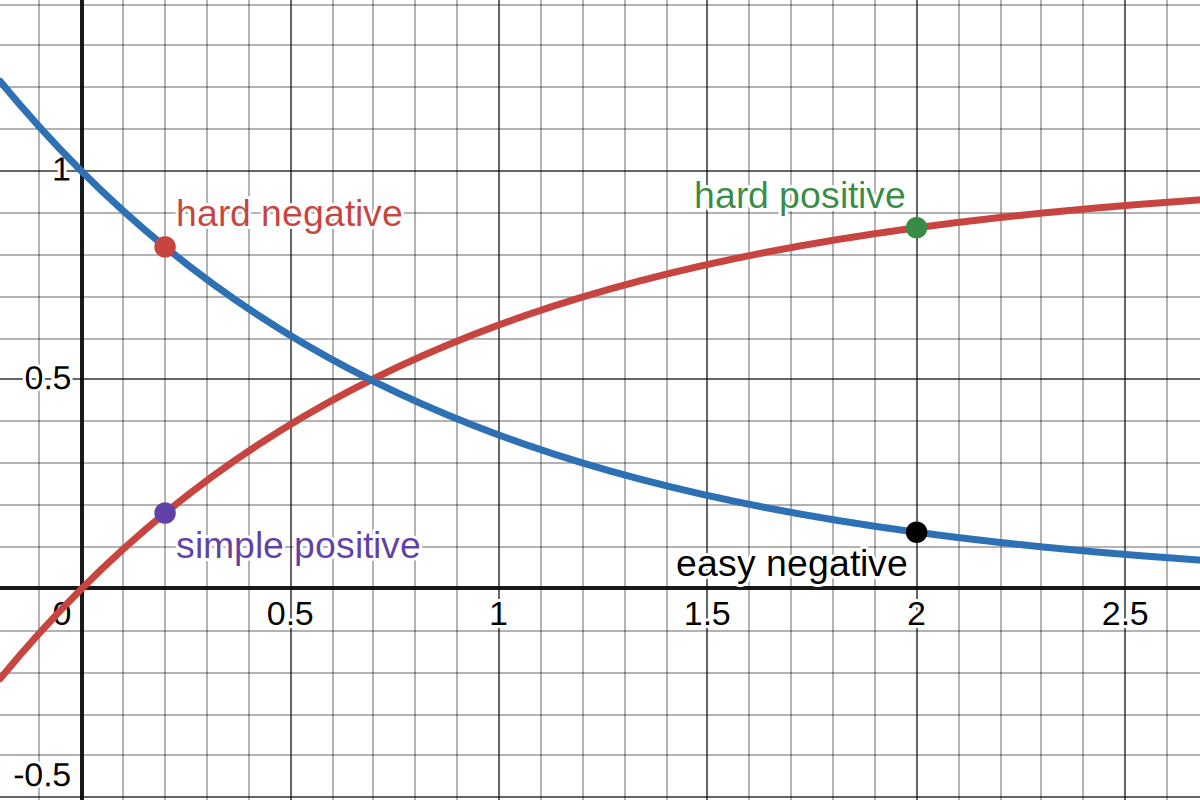
\includegraphics[width=280pt]{images/Hard_easy_samples_dist_effect_loss_desmos.png}
    \caption{The impact of the distance between a generated sample and its anchor on the loss function.
    The red curve represents the loss function for positive samples, 
    whereas the blue curve denotes negative samples.
    Hard samples convey more (gradient) information than easy samples and thus, have a higher loss value.
    While distant positive pairs are considered hard, for negative samples, small proximity ones are considered hard.}
    \label{fig:hard_easy_samples_dist_effect_loss}
\end{figure}


% ---- Bibliography ----
eg \cite{texbook}
\bibliographystyle{splncs04}
\bibliography{references}




\end{document}
